\documentclass{SelimArticle}
\definecolor{RosyBrown}{rgb}{0.737255,0.560784,0.560784}
\definecolor{light goldenrod}{rgb}{0.933333,0.866667,0.509804}
\definecolor{LightGoldenrod}{rgb}{0.933333,0.866667,0.509804}
\definecolor{Sienna}{rgb}{0.627451,0.321569,0.176471}
\definecolor{Red}{rgb}{0.803922,0.000000,0.000000} %Actually red3
%\definecolor{Red}{rgb}{0.803922,0.360784,0.360784} %Actually Indian Red
%\definecolor{Red}{rgb}{0.815686,0.125490,0.564706} %Actually Violet Red
%\definecolor{Red}{rgb}{1.000000,0.270588,0.000000} %Actually Orange Red
%\definecolor{Red}{rgb}{0.545098,0.227451,0.227451} %Actually Indian Red 4
\sectionfont{ \sectionrule{0pt}{0pt}{-5pt}{0.8pt} }  %Horizontal line below section.
\setcounter{secnumdepth}{2}  % Numbering of sections and subsections
\usepackage{pdfpages}
\usepackage[refpage]{nomencl}
\usepackage{multirow}
\usepackage{bigstrut}
\usepackage{pdfpages}
\usepackage{setspace} %allows double spacing with \doublespacing command
\setlength{\nomitemsep}{-\parsep}
\usepackage[linktoc=all]{hyperref} %allows me to make a hyperref table of contents
\hypersetup{
    colorlinks,
    citecolor=black,
    filecolor=black,
    linkcolor=black,
    urlcolor=black
}

%Used for nomenclature making
\renewcommand*{\pagedeclaration}[1]{\unskip\dotfill\hyperpage{#1}}
\makenomenclature
%In CMD, makeindex <filename>.nlo -s nomencl.ist -o <filename>.nls

%%%%%%%%%%%%%%%%%%%%
%EDIT TITLE PAGE%%%%
%\course{Mechanics of Composite Materials}        
%\coursenum{MECH-530} 
%\title{Project - Part 1 \\ Python Code Output}   %Add \\[0.3cm] for other line. 
%\student{Elaine \textsc{Craigie}}  %Simple \\ to add more names. Don't forget \textsc
%\studentnum{260476434}
%\vspace{3cm}
%\date{\today}
%EDIT TITLE PAGE%%%%%
%%%%%%%%%%%%%%%%%%%%%
%%%%%%%%%%%%%%%%%%%%%%%%%%%%%%%%%%%%%%%%%
% Classic Lined Title Page 
% LaTeX Template
% Version 1.0 (27/12/12)
%
% This template has been downloaded from:
% http://www.LaTeXTemplates.com
%
% Original author:
% Peter Wilson (herries.press@earthlink.net)
%
% License:
% CC BY-NC-SA 3.0 (http://creativecommons.org/licenses/by-nc-sa/3.0/)
% 
% Instructions for using this template:
% This title page compiles as is. If you wish to include this title page in 
% another document, you will need to copy everything before 
% \begin{document} into the preamble of your document. The title page is
% then included using \titleAT within your document.
%
%%%%%%%%%%%%%%%%%%%%%%%%%%%%%%%%%%%%%%%%%

%----------------------------------------------------------------------------------------
%	PACKAGES AND OTHER DOCUMENT CONFIGURATIONS
%----------------------------------------------------------------------------------------

\newcommand*{\plogo}{\fbox{$\mathcal{PL}$}} % Generic publisher logo

%----------------------------------------------------------------------------------------
%	TITLE PAGE
%----------------------------------------------------------------------------------------

\newcommand*{\titleAT}{\begingroup % Create the command for including the title page in the document
\newlength{\drop} % Command for generating a specific amount of whitespace
\drop=0.1\textheight % Define the command as 10% of the total text height

\rule{\textwidth}{1pt}\par % Thick horizontal line
\vspace{2pt}\vspace{-\baselineskip} % Whitespace between lines
\rule{\textwidth}{0.4pt}\par % Thin horizontal line

\vspace{\drop} % Whitespace between the top lines and title
\centering % Center all text
\textcolor{Red}{ % Red font color
{\Huge TERM PROJECT}\\[0.5\baselineskip] % Title line 1
{\Large MECH-530}\\[0.75\baselineskip] % Title line 2
{\Huge Progress Report 4}} % Title line 3

\vspace{0.25\drop} % Whitespace between the title and short horizontal line
\rule{0.3\textwidth}{0.4pt}\par % Short horizontal line under the title
\vspace{\drop} % Whitespace between the thin horizontal line and the author name

{\Large \textsc{Elaine Craigie} \\ \vspace{0.5cm} (260476434)}\par % Author name

\vfill % Whitespace between the author name and publisher text
%{\large \textcolor{Red}{\plogo}}\\[0.5\baselineskip] % Publisher logo

\includegraphics[scale = 0.45]{pic_mcgill}
\vspace{2.0cm}
{\Large \textsc{\\ \today}}\par % Publisher
\vspace{1.0cm}
{\raggedleft{}
\textcolor{Red}{
{\large \\ \textsc{Overview:} This progress report features calculating the resultant stress and strain at the top and bottom of each ply in a laminate skateboard to determine if the design criterion are met. New modules include calculating the matrices $D$, $d$, the radius of curvature $K$, as well as developing an input interface for an applied resultant moment $M$.}}}
\centering
\rule{\textwidth}{0.4pt}\par % Thin horizontal line
\vspace{2pt}\vspace{-\baselineskip} % Whitespace between lines
\rule{\textwidth}{1pt}\par % Thick horizontal line

\endgroup}

%----------------------------------------------------------------------------------------
%	BLANK DOCUMENT
%----------------------------------------------------------------------------------------
\begin{document}
\pagestyle{empty} % Removes page numbers

\titleAT % This command includes the title page
%%%%%%%%%%%%%%%%%%%%

%\mytitlepage
%\pagenumbering{roman}
%\setcounter{page}{1}
%\doublespacing
%\tableofcontents
%\newpage
%\renewcommand{\nomname}{List of Symbols}
\printnomenclature[0.5in]
\newpage
\pagenumbering{arabic}
\setcounter{page}{1}
\section{Preliminary Calculations and Design Criterion}
Based on the following given values, $M_{1}$ is determined to be 2869.425~N downwards while $M_{2} = M_{3} = 0$~N
\begin{itemize}
\item L = 52 cm (length of skateboard)
\item b = 10 cm (width of skateboard)
\item m = 225 kg (worst case concentrated mass)
\item W = $225 \cdot 9.81$ = 2207.25 N downwards (worst case concentrated weight) 
\end{itemize}
 
\begin{align*}
M_{1} &= \frac{M}{b} \\
&= \frac{P \cdot b}{4 \cdot b} \\
&= \frac{-225 \cdot 9.81 \cdot 0.52}{4 \cdot 0.1} \\
&= -2869.425 N
\label{eq:appliedload}
\end{align*}

Refer to the end of Section~\ref{sec:programout} for the deflection and the midpoint along with the max strain along the fibers. Note that neither of the following design criterions are met.
\begin{itemize}
\item Max deflection at the skateboard's midpoint: $\delta < 5.0~\text{mm}$
\item Max strain along the fibers: $\epsilon_{x} < 0.002$ 
\end{itemize}

\section{Program Output}
\label{sec:programout}
Program output to follow...
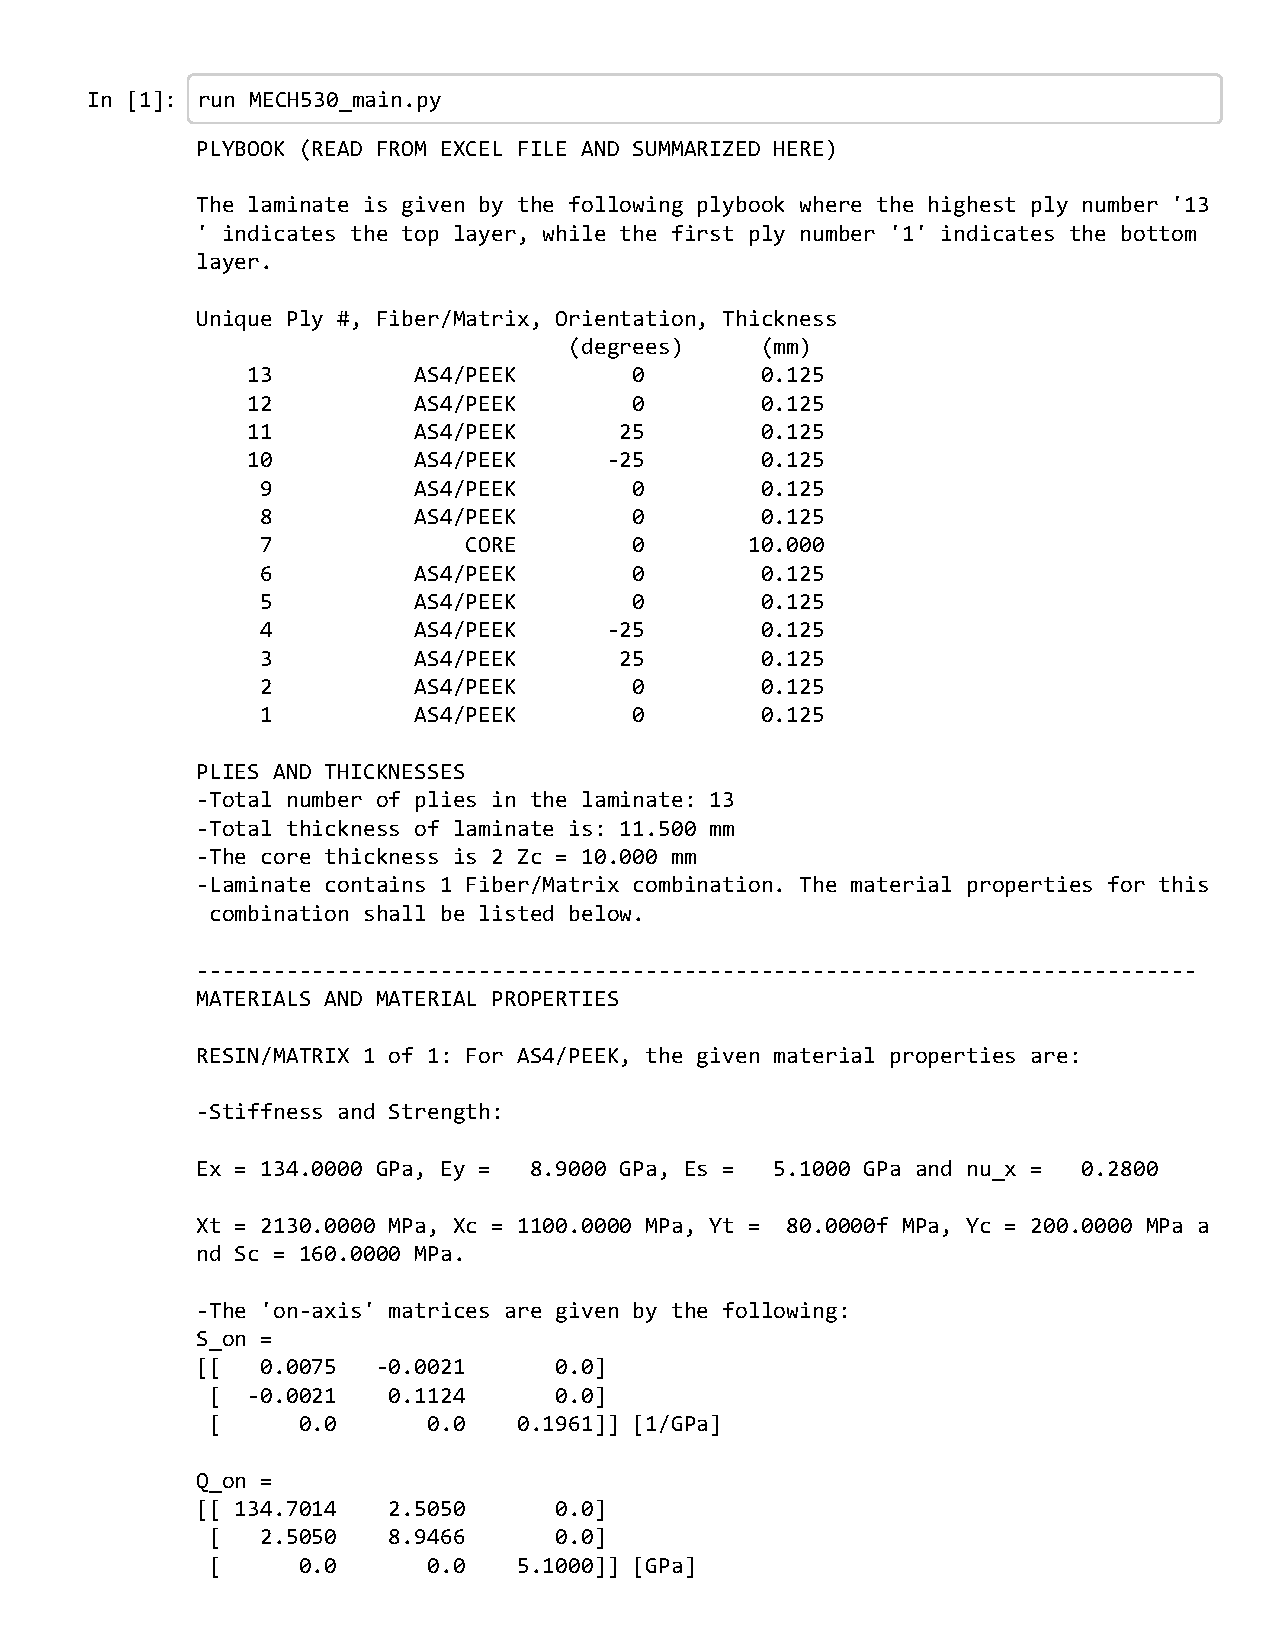
\includepdf[pages={1-8}]{MECH530_Ass4_IPythonNotebook.pdf}

\end{document}